\documentclass[border=12pt]{standalone}
\usepackage{tikz}
\usetikzlibrary{arrows.meta,calc}
\definecolor{basegray}{RGB}{70,78,90}
\definecolor{linkblue}{RGB}{52,98,160}
\definecolor{linkcyan}{RGB}{64,140,170}
\definecolor{jointgold}{RGB}{210,160,50}
\definecolor{axisred}{RGB}{200,60,50}
\definecolor{eeorange}{RGB}{220,120,40}
\definecolor{floorline}{RGB}{180,185,195}
\definecolor{labeldark}{RGB}{40,45,55}
\begin{document}
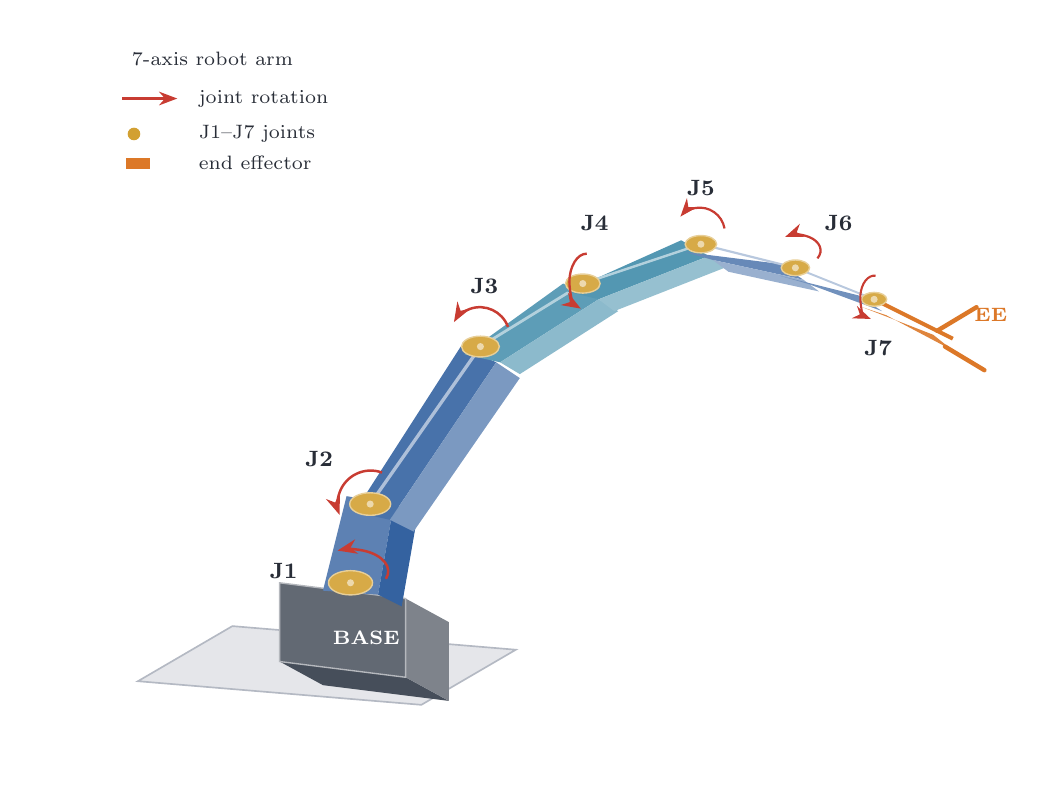
\begin{tikzpicture}[x=1cm,y=1cm,>=Stealth]
  % Viewport ~1200x900 aspect via bounding content
  \clip (-1.2,-1.0) rectangle (11.5,8.6);

  % Floor / base platform (perspective parallelogram)
  \fill[floorline!35]
    (0.2,0.3) -- (3.8,0.0) -- (5.0,0.7) -- (1.4,1.0) -- cycle;
  \draw[floorline,line width=0.6pt]
    (0.2,0.3) -- (3.8,0.0) -- (5.0,0.7) -- (1.4,1.0) -- cycle;

  % --- Base pedestal ---
  \fill[basegray!85]
    (2.0,0.55) -- (3.6,0.35) -- (3.6,1.35) -- (2.0,1.55) -- cycle;
  \fill[basegray]
    (2.0,0.55) -- (2.55,0.25) -- (4.15,0.05) -- (3.6,0.35) -- cycle;
  \fill[basegray!70]
    (3.6,0.35) -- (4.15,0.05) -- (4.15,1.05) -- (3.6,1.35) -- cycle;
  \draw[basegray!40,line width=0.5pt]
    (2.0,0.55) -- (3.6,0.35) -- (3.6,1.35) -- (2.0,1.55) -- cycle;
  \node[font=\scriptsize\bfseries,text=white] at (3.1,0.85) {BASE};

  % Joint centers (isometric-ish side elevation)
  % J1: yaw on base
  \coordinate (J1) at (2.9,1.55);
  % J2: shoulder pitch
  \coordinate (J2) at (3.15,2.55);
  % J3: elbow pitch
  \coordinate (J3) at (4.55,4.55);
  % J4: forearm roll
  \coordinate (J4) at (5.85,5.35);
  % J5: wrist pitch
  \coordinate (J5) at (7.35,5.85);
  % J6: wrist yaw
  \coordinate (J6) at (8.55,5.55);
  % J7: tool roll / flange
  \coordinate (J7) at (9.55,5.15);
  % End effector tip
  \coordinate (EE) at (10.55,4.65);

  % --- Link 0: base column to J1/J2 ---
  \fill[linkblue!80]
    (2.55,1.45) -- (3.25,1.40) -- (3.45,2.55) -- (2.85,2.65) -- cycle;
  \fill[linkblue]
    (3.25,1.40) -- (3.55,1.25) -- (3.75,2.40) -- (3.45,2.55) -- cycle;

  % --- Link 1: upper arm J2--J3 ---
  \fill[linkblue!90]
    (2.95,2.45) -- (3.40,2.35) -- (4.75,4.35) -- (4.30,4.55) -- cycle;
  \fill[linkblue!65]
    (3.40,2.35) -- (3.70,2.20) -- (5.05,4.15) -- (4.75,4.35) -- cycle;
  \draw[linkblue!40,line width=1.2pt] (J2) -- (J3);

  % --- Link 2: forearm J3--J4 ---
  \fill[linkcyan!85]
    (4.35,4.45) -- (4.80,4.35) -- (6.05,5.15) -- (5.60,5.35) -- cycle;
  \fill[linkcyan!60]
    (4.80,4.35) -- (5.05,4.20) -- (6.30,5.00) -- (6.05,5.15) -- cycle;
  \draw[linkcyan!40,line width=1.0pt] (J3) -- (J4);

  % --- Link 3: wrist proximal J4--J5 ---
  \fill[linkcyan!90]
    (5.65,5.25) -- (6.05,5.15) -- (7.45,5.70) -- (7.10,5.90) -- cycle;
  \fill[linkcyan!55]
    (6.05,5.15) -- (6.25,5.00) -- (7.65,5.55) -- (7.45,5.70) -- cycle;
  \draw[linkcyan!40,line width=0.9pt] (J4) -- (J5);

  % --- Link 4: wrist distal J5--J6 ---
  \fill[linkblue!75]
    (7.15,5.75) -- (7.50,5.65) -- (8.65,5.40) -- (8.35,5.60) -- cycle;
  \fill[linkblue!50]
    (7.50,5.65) -- (7.70,5.50) -- (8.85,5.25) -- (8.65,5.40) -- cycle;
  \draw[linkblue!35,line width=0.8pt] (J5) -- (J6);

  % --- Link 5: flange J6--J7 ---
  \fill[linkblue!70]
    (8.35,5.45) -- (8.70,5.35) -- (9.65,5.00) -- (9.35,5.20) -- cycle;
  \draw[linkblue!35,line width=0.7pt] (J6) -- (J7);

  % --- End effector / gripper ---
  \fill[eeorange!90]
    (9.40,5.05) -- (9.70,4.95) -- (10.55,4.50) -- (10.30,4.70) -- cycle;
  \draw[eeorange,line width=1.4pt] (J7) -- (EE);
  % Fingers
  \draw[eeorange,line width=1.6pt,line cap=round]
    (10.35,4.75) -- (10.85,5.05);
  \draw[eeorange,line width=1.6pt,line cap=round]
    (10.45,4.55) -- (10.95,4.25);
  \node[font=\scriptsize\bfseries,text=eeorange,anchor=west] at (10.7,4.95) {EE};

  % --- Joint disks (ellipses for 3D) ---
  \foreach \P/\s in {J1/0.28,J2/0.26,J3/0.24,J4/0.22,J5/0.20,J6/0.18,J7/0.16} {
    \fill[jointgold!90] (\P) ellipse [x radius=\s, y radius=\s*0.55];
    \draw[jointgold!50,line width=0.5pt] (\P) ellipse [x radius=\s, y radius=\s*0.55];
    \fill[jointgold!40] (\P) circle [radius=0.045];
  }

  % --- Axis rotation arrows (curved) + labels ---
  % J1 yaw (vertical axis) — arc around J1
  \draw[axisred,->,line width=0.9pt]
    ([shift={(0.45,0.05)}]J1) arc [start angle=-20, end angle=110, x radius=0.48, y radius=0.28];
  \node[font=\footnotesize\bfseries,text=labeldark,anchor=east] at ([shift={(-0.55,0.15)}]J1) {J1};

  % J2 pitch
  \draw[axisred,->,line width=0.9pt]
    ([shift={(0.15,0.40)}]J2) arc [start angle=70, end angle=200, radius=0.42];
  \node[font=\footnotesize\bfseries,text=labeldark,anchor=south east] at ([shift={(-0.35,0.35)}]J2) {J2};

  % J3 pitch
  \draw[axisred,->,line width=0.9pt]
    ([shift={(0.35,0.25)}]J3) arc [start angle=20, end angle=150, radius=0.38];
  \node[font=\footnotesize\bfseries,text=labeldark,anchor=south] at ([shift={(0.05,0.55)}]J3) {J3};

  % J4 roll (along forearm)
  \draw[axisred,->,line width=0.85pt]
    ([shift={(0.05,0.38)}]J4) arc [start angle=90, end angle=250, x radius=0.22, y radius=0.36];
  \node[font=\footnotesize\bfseries,text=labeldark,anchor=south] at ([shift={(0.15,0.55)}]J4) {J4};

  % J5 pitch
  \draw[axisred,->,line width=0.8pt]
    ([shift={(0.30,0.20)}]J5) arc [start angle=10, end angle=140, radius=0.32];
  \node[font=\footnotesize\bfseries,text=labeldark,anchor=south] at ([shift={(0.0,0.50)}]J5) {J5};

  % J6 yaw
  \draw[axisred,->,line width=0.8pt]
    ([shift={(0.28,0.12)}]J6) arc [start angle=-30, end angle=120, x radius=0.30, y radius=0.20];
  \node[font=\footnotesize\bfseries,text=labeldark,anchor=south west] at ([shift={(0.25,0.35)}]J6) {J6};

  % J7 tool roll
  \draw[axisred,->,line width=0.75pt]
    ([shift={(0.02,0.30)}]J7) arc [start angle=85, end angle=255, x radius=0.18, y radius=0.28];
  \node[font=\footnotesize\bfseries,text=labeldark,anchor=north] at ([shift={(0.05,-0.40)}]J7) {J7};

  % Legend
  \node[font=\scriptsize,text=labeldark,anchor=west] at (0.0,8.2) {7-axis robot arm};
  \draw[axisred,->,line width=0.8pt] (0.0,7.7) -- (0.7,7.7);
  \node[font=\scriptsize,text=labeldark,anchor=west] at (0.85,7.7) {joint rotation};
  \fill[jointgold] (0.15,7.25) circle [radius=0.08];
  \node[font=\scriptsize,text=labeldark,anchor=west] at (0.85,7.25) {J1--J7 joints};
  \fill[eeorange] (0.05,6.80) rectangle (0.35,6.95);
  \node[font=\scriptsize,text=labeldark,anchor=west] at (0.85,6.88) {end effector};

\end{tikzpicture}
\end{document}
